% Goodstein sequences (generated by figs_c3ch07.py).
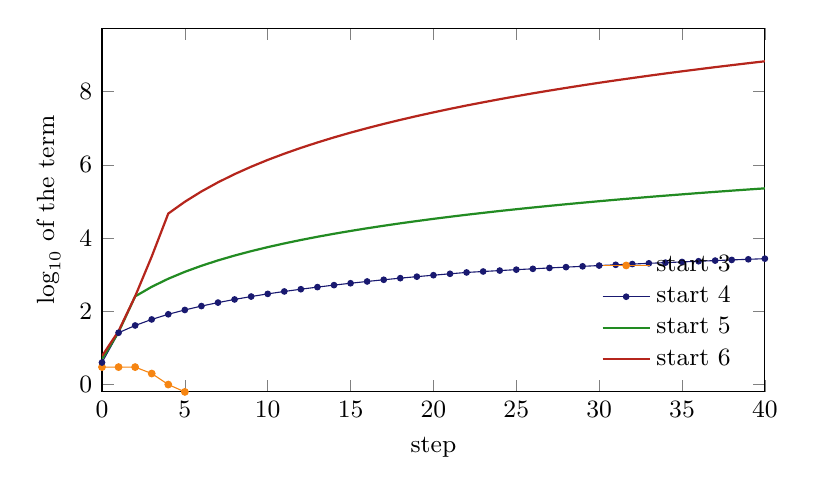
\begin{tikzpicture}
\begin{axis}[width=10cm,height=6.2cm,xlabel={step},ylabel={$\log_{10}$ of the term},xmin=0,xmax=40,ymin=-0.2,
  legend pos=south east,legend style={font=\small,draw=none,fill=none},tick label style={font=\small},label style={font=\small}]
\addplot[BurntOrange,mark=*,mark size=1.2pt] coordinates {(0,0.477) (1,0.477) (2,0.477) (3,0.301) (4,0.000) (5,-0.200)};
\addlegendentry{start $3$}
\addplot[MidnightBlue,mark=*,mark size=1pt] coordinates {(0,0.602) (1,1.415) (2,1.613) (3,1.778) (4,1.919) (5,2.037) (6,2.143) (7,2.238) (8,2.324) (9,2.403) (10,2.476) (11,2.542) (12,2.603) (13,2.661) (14,2.715) (15,2.766) (16,2.815) (17,2.861) (18,2.905) (19,2.946) (20,2.986) (21,3.024) (22,3.061) (23,3.087) (24,3.112) (25,3.137) (26,3.160) (27,3.184) (28,3.206) (29,3.228) (30,3.249) (31,3.270) (32,3.290) (33,3.310) (34,3.329) (35,3.348) (36,3.367) (37,3.385) (38,3.403) (39,3.420) (40,3.437)};
\addlegendentry{start $4$}
\addplot[ForestGreen,thick] coordinates {(0,0.699) (1,1.431) (2,2.407) (3,2.669) (4,2.889) (5,3.078) (6,3.243) (7,3.390) (8,3.522) (9,3.642) (10,3.752) (11,3.853) (12,3.947) (13,4.035) (14,4.117) (15,4.194) (16,4.267) (17,4.336) (18,4.402) (19,4.464) (20,4.524) (21,4.581) (22,4.636) (23,4.688) (24,4.739) (25,4.787) (26,4.834) (27,4.879) (28,4.923) (29,4.965) (30,5.006) (31,5.046) (32,5.084) (33,5.122) (34,5.158) (35,5.193) (36,5.228) (37,5.261) (38,5.294) (39,5.326) (40,5.357)};
\addlegendentry{start $5$}
\addplot[BrickRed,thick] coordinates {(0,0.778) (1,1.462) (2,2.410) (3,3.495) (4,4.669) (5,4.991) (6,5.272) (7,5.521) (8,5.745) (9,5.947) (10,6.133) (11,6.303) (12,6.462) (13,6.609) (14,6.748) (15,6.878) (16,7.000) (17,7.116) (18,7.226) (19,7.331) (20,7.431) (21,7.527) (22,7.619) (23,7.706) (24,7.791) (25,7.872) (26,7.951) (27,8.026) (28,8.099) (29,8.170) (30,8.239) (31,8.305) (32,8.369) (33,8.432) (34,8.493) (35,8.552) (36,8.609) (37,8.666) (38,8.720) (39,8.774) (40,8.826)};
\addlegendentry{start $6$}
\end{axis}
\end{tikzpicture}
